% Created by tikzDevice version 0.6.1 on 2016-04-19 18:41:22
% !TEX encoding = UTF-8 Unicode
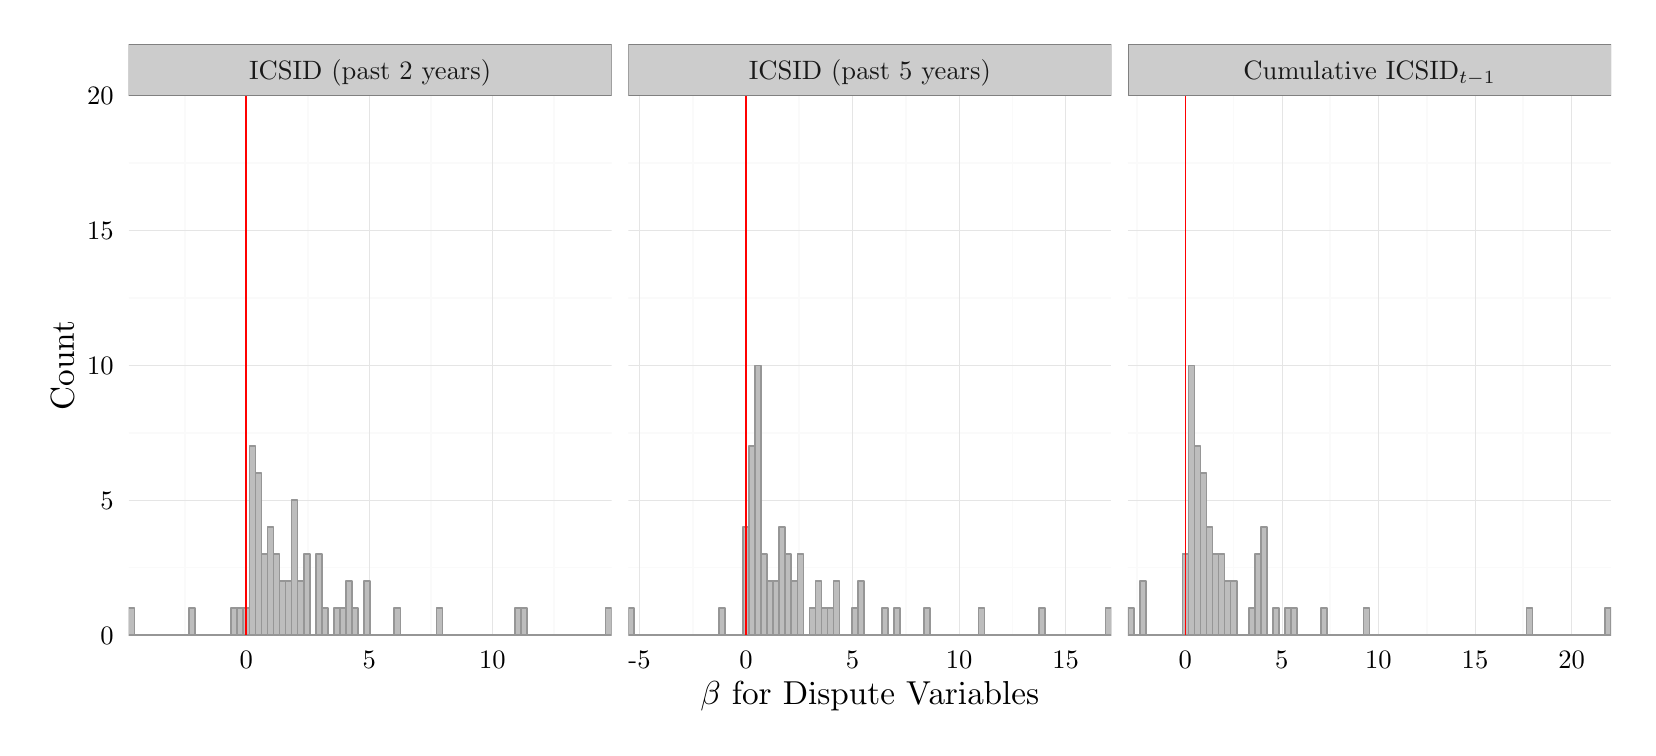
\begin{tikzpicture}[x=1pt,y=1pt]
\definecolor[named]{drawColor}{rgb}{0.00,0.00,0.00}
\definecolor[named]{fillColor}{rgb}{1.00,1.00,1.00}
\fill[color=fillColor,] (0,0) rectangle (578.16,252.94);
\begin{scope}
\path[clip] (  0.00,  0.00) rectangle (578.16,252.94);
\end{scope}
\begin{scope}
\path[clip] (  0.00,  0.00) rectangle (578.16,252.94);
\end{scope}
\begin{scope}
\path[clip] (  0.00,  0.00) rectangle (578.16,252.94);
\end{scope}
\begin{scope}
\path[clip] (  0.00,  0.00) rectangle (578.16,252.94);
\end{scope}
\begin{scope}
\path[clip] (  0.00,  0.00) rectangle (578.16,252.94);
\end{scope}
\begin{scope}
\path[clip] (  0.00,  0.00) rectangle (578.16,252.94);
\end{scope}
\begin{scope}
\path[clip] (  0.00,  0.00) rectangle (578.16,252.94);
\end{scope}
\begin{scope}
\path[clip] (  0.00,  0.00) rectangle (578.16,252.94);
\end{scope}
\begin{scope}
\path[clip] (  0.00,  0.00) rectangle (578.16,252.94);
\end{scope}
\begin{scope}
\path[clip] (  0.00,  0.00) rectangle (578.16,252.94);
\end{scope}
\begin{scope}
\path[clip] (  0.00,  0.00) rectangle (578.16,252.94);
\end{scope}
\begin{scope}
\path[clip] (  0.00,  0.00) rectangle (578.16,252.94);
\end{scope}
\begin{scope}
\path[clip] (  0.00,  0.00) rectangle (578.16,252.94);
\end{scope}
\begin{scope}
\path[clip] (  0.00,  0.00) rectangle (578.16,252.94);
\end{scope}
\begin{scope}
\path[clip] (  0.00,  0.00) rectangle (578.16,252.94);
\end{scope}
\begin{scope}
\path[clip] (  0.00,  0.00) rectangle (578.16,252.94);
\end{scope}
\begin{scope}
\path[clip] (  0.00,  0.00) rectangle (578.16,252.94);
\definecolor[named]{drawColor}{rgb}{1.00,1.00,1.00}
\definecolor[named]{fillColor}{rgb}{1.00,1.00,1.00}

\draw[color=drawColor,line width= 0.6pt,line cap=round,line join=round,fill=fillColor,] (  0.00,  0.00) rectangle (578.16,252.95);
\end{scope}
\begin{scope}
\path[clip] (  0.00,  0.00) rectangle (578.16,252.94);
\end{scope}
\begin{scope}
\path[clip] ( 36.46, 33.48) rectangle (211.03,228.33);
\definecolor[named]{fillColor}{rgb}{1.00,1.00,1.00}

\draw[fill=fillColor,draw opacity=0.00,] ( 36.46, 33.48) rectangle (211.03,228.33);
\definecolor[named]{drawColor}{rgb}{0.98,0.98,0.98}

\draw[color=drawColor,line width= 0.6pt,line join=round,fill opacity=0.00,] ( 36.46, 57.83) --
	(211.03, 57.83);

\draw[color=drawColor,line width= 0.6pt,line join=round,fill opacity=0.00,] ( 36.46,106.55) --
	(211.03,106.55);

\draw[color=drawColor,line width= 0.6pt,line join=round,fill opacity=0.00,] ( 36.46,155.26) --
	(211.03,155.26);

\draw[color=drawColor,line width= 0.6pt,line join=round,fill opacity=0.00,] ( 36.46,203.98) --
	(211.03,203.98);

\draw[color=drawColor,line width= 0.6pt,line join=round,fill opacity=0.00,] ( 56.79, 33.48) --
	( 56.79,228.33);

\draw[color=drawColor,line width= 0.6pt,line join=round,fill opacity=0.00,] (101.23, 33.48) --
	(101.23,228.33);

\draw[color=drawColor,line width= 0.6pt,line join=round,fill opacity=0.00,] (145.67, 33.48) --
	(145.67,228.33);

\draw[color=drawColor,line width= 0.6pt,line join=round,fill opacity=0.00,] (190.11, 33.48) --
	(190.11,228.33);
\definecolor[named]{drawColor}{rgb}{0.90,0.90,0.90}

\draw[color=drawColor,line width= 0.2pt,line join=round,fill opacity=0.00,] ( 36.46, 33.48) --
	(211.03, 33.48);

\draw[color=drawColor,line width= 0.2pt,line join=round,fill opacity=0.00,] ( 36.46, 82.19) --
	(211.03, 82.19);

\draw[color=drawColor,line width= 0.2pt,line join=round,fill opacity=0.00,] ( 36.46,130.90) --
	(211.03,130.90);

\draw[color=drawColor,line width= 0.2pt,line join=round,fill opacity=0.00,] ( 36.46,179.62) --
	(211.03,179.62);

\draw[color=drawColor,line width= 0.2pt,line join=round,fill opacity=0.00,] ( 36.46,228.33) --
	(211.03,228.33);

\draw[color=drawColor,line width= 0.2pt,line join=round,fill opacity=0.00,] ( 79.01, 33.48) --
	( 79.01,228.33);

\draw[color=drawColor,line width= 0.2pt,line join=round,fill opacity=0.00,] (123.45, 33.48) --
	(123.45,228.33);

\draw[color=drawColor,line width= 0.2pt,line join=round,fill opacity=0.00,] (167.89, 33.48) --
	(167.89,228.33);
\definecolor[named]{drawColor}{rgb}{0.59,0.59,0.59}
\definecolor[named]{fillColor}{rgb}{0.74,0.74,0.74}

\draw[color=drawColor,line width= 0.6pt,line join=round,fill=fillColor,] ( 36.46, 33.48) rectangle ( 38.64, 43.22);

\draw[color=drawColor,line width= 0.6pt,line join=round,fill=fillColor,] ( 38.64, 33.48) rectangle ( 40.83, 33.48);

\draw[color=drawColor,line width= 0.6pt,line join=round,fill=fillColor,] ( 40.83, 33.48) rectangle ( 43.01, 33.48);

\draw[color=drawColor,line width= 0.6pt,line join=round,fill=fillColor,] ( 43.01, 33.48) rectangle ( 45.19, 33.48);

\draw[color=drawColor,line width= 0.6pt,line join=round,fill=fillColor,] ( 45.19, 33.48) rectangle ( 47.37, 33.48);

\draw[color=drawColor,line width= 0.6pt,line join=round,fill=fillColor,] ( 47.37, 33.48) rectangle ( 49.55, 33.48);

\draw[color=drawColor,line width= 0.6pt,line join=round,fill=fillColor,] ( 49.55, 33.48) rectangle ( 51.74, 33.48);

\draw[color=drawColor,line width= 0.6pt,line join=round,fill=fillColor,] ( 51.74, 33.48) rectangle ( 53.92, 33.48);

\draw[color=drawColor,line width= 0.6pt,line join=round,fill=fillColor,] ( 53.92, 33.48) rectangle ( 56.10, 33.48);

\draw[color=drawColor,line width= 0.6pt,line join=round,fill=fillColor,] ( 56.10, 33.48) rectangle ( 58.28, 33.48);

\draw[color=drawColor,line width= 0.6pt,line join=round,fill=fillColor,] ( 58.28, 33.48) rectangle ( 60.47, 43.22);

\draw[color=drawColor,line width= 0.6pt,line join=round,fill=fillColor,] ( 60.47, 33.48) rectangle ( 62.65, 33.48);

\draw[color=drawColor,line width= 0.6pt,line join=round,fill=fillColor,] ( 62.65, 33.48) rectangle ( 64.83, 33.48);

\draw[color=drawColor,line width= 0.6pt,line join=round,fill=fillColor,] ( 64.83, 33.48) rectangle ( 67.01, 33.48);

\draw[color=drawColor,line width= 0.6pt,line join=round,fill=fillColor,] ( 67.01, 33.48) rectangle ( 69.19, 33.48);

\draw[color=drawColor,line width= 0.6pt,line join=round,fill=fillColor,] ( 69.19, 33.48) rectangle ( 71.38, 33.48);

\draw[color=drawColor,line width= 0.6pt,line join=round,fill=fillColor,] ( 71.38, 33.48) rectangle ( 73.56, 33.48);

\draw[color=drawColor,line width= 0.6pt,line join=round,fill=fillColor,] ( 73.56, 33.48) rectangle ( 75.74, 43.22);

\draw[color=drawColor,line width= 0.6pt,line join=round,fill=fillColor,] ( 75.74, 33.48) rectangle ( 77.92, 43.22);

\draw[color=drawColor,line width= 0.6pt,line join=round,fill=fillColor,] ( 77.92, 33.48) rectangle ( 80.10, 43.22);

\draw[color=drawColor,line width= 0.6pt,line join=round,fill=fillColor,] ( 80.10, 33.48) rectangle ( 82.29,101.68);

\draw[color=drawColor,line width= 0.6pt,line join=round,fill=fillColor,] ( 82.29, 33.48) rectangle ( 84.47, 91.93);

\draw[color=drawColor,line width= 0.6pt,line join=round,fill=fillColor,] ( 84.47, 33.48) rectangle ( 86.65, 62.70);

\draw[color=drawColor,line width= 0.6pt,line join=round,fill=fillColor,] ( 86.65, 33.48) rectangle ( 88.83, 72.45);

\draw[color=drawColor,line width= 0.6pt,line join=round,fill=fillColor,] ( 88.83, 33.48) rectangle ( 91.01, 62.70);

\draw[color=drawColor,line width= 0.6pt,line join=round,fill=fillColor,] ( 91.01, 33.48) rectangle ( 93.20, 52.96);

\draw[color=drawColor,line width= 0.6pt,line join=round,fill=fillColor,] ( 93.20, 33.48) rectangle ( 95.38, 52.96);

\draw[color=drawColor,line width= 0.6pt,line join=round,fill=fillColor,] ( 95.38, 33.48) rectangle ( 97.56, 82.19);

\draw[color=drawColor,line width= 0.6pt,line join=round,fill=fillColor,] ( 97.56, 33.48) rectangle ( 99.74, 52.96);

\draw[color=drawColor,line width= 0.6pt,line join=round,fill=fillColor,] ( 99.74, 33.48) rectangle (101.92, 62.70);

\draw[color=drawColor,line width= 0.6pt,line join=round,fill=fillColor,] (101.92, 33.48) rectangle (104.11, 33.48);

\draw[color=drawColor,line width= 0.6pt,line join=round,fill=fillColor,] (104.11, 33.48) rectangle (106.29, 62.70);

\draw[color=drawColor,line width= 0.6pt,line join=round,fill=fillColor,] (106.29, 33.48) rectangle (108.47, 43.22);

\draw[color=drawColor,line width= 0.6pt,line join=round,fill=fillColor,] (108.47, 33.48) rectangle (110.65, 33.48);

\draw[color=drawColor,line width= 0.6pt,line join=round,fill=fillColor,] (110.65, 33.48) rectangle (112.83, 43.22);

\draw[color=drawColor,line width= 0.6pt,line join=round,fill=fillColor,] (112.83, 33.48) rectangle (115.02, 43.22);

\draw[color=drawColor,line width= 0.6pt,line join=round,fill=fillColor,] (115.02, 33.48) rectangle (117.20, 52.96);

\draw[color=drawColor,line width= 0.6pt,line join=round,fill=fillColor,] (117.20, 33.48) rectangle (119.38, 43.22);

\draw[color=drawColor,line width= 0.6pt,line join=round,fill=fillColor,] (119.38, 33.48) rectangle (121.56, 33.48);

\draw[color=drawColor,line width= 0.6pt,line join=round,fill=fillColor,] (121.56, 33.48) rectangle (123.75, 52.96);

\draw[color=drawColor,line width= 0.6pt,line join=round,fill=fillColor,] (123.75, 33.48) rectangle (125.93, 33.48);

\draw[color=drawColor,line width= 0.6pt,line join=round,fill=fillColor,] (125.93, 33.48) rectangle (128.11, 33.48);

\draw[color=drawColor,line width= 0.6pt,line join=round,fill=fillColor,] (128.11, 33.48) rectangle (130.29, 33.48);

\draw[color=drawColor,line width= 0.6pt,line join=round,fill=fillColor,] (130.29, 33.48) rectangle (132.47, 33.48);

\draw[color=drawColor,line width= 0.6pt,line join=round,fill=fillColor,] (132.47, 33.48) rectangle (134.66, 43.22);

\draw[color=drawColor,line width= 0.6pt,line join=round,fill=fillColor,] (134.66, 33.48) rectangle (136.84, 33.48);

\draw[color=drawColor,line width= 0.6pt,line join=round,fill=fillColor,] (136.84, 33.48) rectangle (139.02, 33.48);

\draw[color=drawColor,line width= 0.6pt,line join=round,fill=fillColor,] (139.02, 33.48) rectangle (141.20, 33.48);

\draw[color=drawColor,line width= 0.6pt,line join=round,fill=fillColor,] (141.20, 33.48) rectangle (143.38, 33.48);

\draw[color=drawColor,line width= 0.6pt,line join=round,fill=fillColor,] (143.38, 33.48) rectangle (145.57, 33.48);

\draw[color=drawColor,line width= 0.6pt,line join=round,fill=fillColor,] (145.57, 33.48) rectangle (147.75, 33.48);

\draw[color=drawColor,line width= 0.6pt,line join=round,fill=fillColor,] (147.75, 33.48) rectangle (149.93, 43.22);

\draw[color=drawColor,line width= 0.6pt,line join=round,fill=fillColor,] (149.93, 33.48) rectangle (152.11, 33.48);

\draw[color=drawColor,line width= 0.6pt,line join=round,fill=fillColor,] (152.11, 33.48) rectangle (154.29, 33.48);

\draw[color=drawColor,line width= 0.6pt,line join=round,fill=fillColor,] (154.29, 33.48) rectangle (156.48, 33.48);

\draw[color=drawColor,line width= 0.6pt,line join=round,fill=fillColor,] (156.48, 33.48) rectangle (158.66, 33.48);

\draw[color=drawColor,line width= 0.6pt,line join=round,fill=fillColor,] (158.66, 33.48) rectangle (160.84, 33.48);

\draw[color=drawColor,line width= 0.6pt,line join=round,fill=fillColor,] (160.84, 33.48) rectangle (163.02, 33.48);

\draw[color=drawColor,line width= 0.6pt,line join=round,fill=fillColor,] (163.02, 33.48) rectangle (165.20, 33.48);

\draw[color=drawColor,line width= 0.6pt,line join=round,fill=fillColor,] (165.20, 33.48) rectangle (167.39, 33.48);

\draw[color=drawColor,line width= 0.6pt,line join=round,fill=fillColor,] (167.39, 33.48) rectangle (169.57, 33.48);

\draw[color=drawColor,line width= 0.6pt,line join=round,fill=fillColor,] (169.57, 33.48) rectangle (171.75, 33.48);

\draw[color=drawColor,line width= 0.6pt,line join=round,fill=fillColor,] (171.75, 33.48) rectangle (173.93, 33.48);

\draw[color=drawColor,line width= 0.6pt,line join=round,fill=fillColor,] (173.93, 33.48) rectangle (176.12, 33.48);

\draw[color=drawColor,line width= 0.6pt,line join=round,fill=fillColor,] (176.12, 33.48) rectangle (178.30, 43.22);

\draw[color=drawColor,line width= 0.6pt,line join=round,fill=fillColor,] (178.30, 33.48) rectangle (180.48, 43.22);

\draw[color=drawColor,line width= 0.6pt,line join=round,fill=fillColor,] (180.48, 33.48) rectangle (182.66, 33.48);

\draw[color=drawColor,line width= 0.6pt,line join=round,fill=fillColor,] (182.66, 33.48) rectangle (184.84, 33.48);

\draw[color=drawColor,line width= 0.6pt,line join=round,fill=fillColor,] (184.84, 33.48) rectangle (187.03, 33.48);

\draw[color=drawColor,line width= 0.6pt,line join=round,fill=fillColor,] (187.03, 33.48) rectangle (189.21, 33.48);

\draw[color=drawColor,line width= 0.6pt,line join=round,fill=fillColor,] (189.21, 33.48) rectangle (191.39, 33.48);

\draw[color=drawColor,line width= 0.6pt,line join=round,fill=fillColor,] (191.39, 33.48) rectangle (193.57, 33.48);

\draw[color=drawColor,line width= 0.6pt,line join=round,fill=fillColor,] (193.57, 33.48) rectangle (195.75, 33.48);

\draw[color=drawColor,line width= 0.6pt,line join=round,fill=fillColor,] (195.75, 33.48) rectangle (197.94, 33.48);

\draw[color=drawColor,line width= 0.6pt,line join=round,fill=fillColor,] (197.94, 33.48) rectangle (200.12, 33.48);

\draw[color=drawColor,line width= 0.6pt,line join=round,fill=fillColor,] (200.12, 33.48) rectangle (202.30, 33.48);

\draw[color=drawColor,line width= 0.6pt,line join=round,fill=fillColor,] (202.30, 33.48) rectangle (204.48, 33.48);

\draw[color=drawColor,line width= 0.6pt,line join=round,fill=fillColor,] (204.48, 33.48) rectangle (206.66, 33.48);

\draw[color=drawColor,line width= 0.6pt,line join=round,fill=fillColor,] (206.66, 33.48) rectangle (208.85, 33.48);

\draw[color=drawColor,line width= 0.6pt,line join=round,fill=fillColor,] (208.85, 33.48) rectangle (211.03, 43.22);
\definecolor[named]{drawColor}{rgb}{1.00,0.00,0.00}
\definecolor[named]{fillColor}{rgb}{1.00,0.00,0.00}

\draw[color=drawColor,line width= 0.6pt,line join=round,fill=fillColor,] ( 79.01, 33.48) -- ( 79.01,228.33);
\end{scope}
\begin{scope}
\path[clip] (  0.00,  0.00) rectangle (578.16,252.94);
\end{scope}
\begin{scope}
\path[clip] (217.03, 33.48) rectangle (391.59,228.33);
\definecolor[named]{fillColor}{rgb}{1.00,1.00,1.00}

\draw[fill=fillColor,draw opacity=0.00,] (217.03, 33.48) rectangle (391.59,228.33);
\definecolor[named]{drawColor}{rgb}{0.98,0.98,0.98}

\draw[color=drawColor,line width= 0.6pt,line join=round,fill opacity=0.00,] (217.03, 57.83) --
	(391.59, 57.83);

\draw[color=drawColor,line width= 0.6pt,line join=round,fill opacity=0.00,] (217.03,106.55) --
	(391.59,106.55);

\draw[color=drawColor,line width= 0.6pt,line join=round,fill opacity=0.00,] (217.03,155.26) --
	(391.59,155.26);

\draw[color=drawColor,line width= 0.6pt,line join=round,fill opacity=0.00,] (217.03,203.98) --
	(391.59,203.98);

\draw[color=drawColor,line width= 0.6pt,line join=round,fill opacity=0.00,] (240.33, 33.48) --
	(240.33,228.33);

\draw[color=drawColor,line width= 0.6pt,line join=round,fill opacity=0.00,] (278.83, 33.48) --
	(278.83,228.33);

\draw[color=drawColor,line width= 0.6pt,line join=round,fill opacity=0.00,] (317.33, 33.48) --
	(317.33,228.33);

\draw[color=drawColor,line width= 0.6pt,line join=round,fill opacity=0.00,] (355.83, 33.48) --
	(355.83,228.33);
\definecolor[named]{drawColor}{rgb}{0.90,0.90,0.90}

\draw[color=drawColor,line width= 0.2pt,line join=round,fill opacity=0.00,] (217.03, 33.48) --
	(391.59, 33.48);

\draw[color=drawColor,line width= 0.2pt,line join=round,fill opacity=0.00,] (217.03, 82.19) --
	(391.59, 82.19);

\draw[color=drawColor,line width= 0.2pt,line join=round,fill opacity=0.00,] (217.03,130.90) --
	(391.59,130.90);

\draw[color=drawColor,line width= 0.2pt,line join=round,fill opacity=0.00,] (217.03,179.62) --
	(391.59,179.62);

\draw[color=drawColor,line width= 0.2pt,line join=round,fill opacity=0.00,] (217.03,228.33) --
	(391.59,228.33);

\draw[color=drawColor,line width= 0.2pt,line join=round,fill opacity=0.00,] (221.08, 33.48) --
	(221.08,228.33);

\draw[color=drawColor,line width= 0.2pt,line join=round,fill opacity=0.00,] (259.58, 33.48) --
	(259.58,228.33);

\draw[color=drawColor,line width= 0.2pt,line join=round,fill opacity=0.00,] (298.08, 33.48) --
	(298.08,228.33);

\draw[color=drawColor,line width= 0.2pt,line join=round,fill opacity=0.00,] (336.58, 33.48) --
	(336.58,228.33);

\draw[color=drawColor,line width= 0.2pt,line join=round,fill opacity=0.00,] (375.08, 33.48) --
	(375.08,228.33);
\definecolor[named]{drawColor}{rgb}{0.59,0.59,0.59}
\definecolor[named]{fillColor}{rgb}{0.74,0.74,0.74}

\draw[color=drawColor,line width= 0.6pt,line join=round,fill=fillColor,] (217.03, 33.48) rectangle (219.21, 43.22);

\draw[color=drawColor,line width= 0.6pt,line join=round,fill=fillColor,] (219.21, 33.48) rectangle (221.39, 33.48);

\draw[color=drawColor,line width= 0.6pt,line join=round,fill=fillColor,] (221.39, 33.48) rectangle (223.57, 33.48);

\draw[color=drawColor,line width= 0.6pt,line join=round,fill=fillColor,] (223.57, 33.48) rectangle (225.76, 33.48);

\draw[color=drawColor,line width= 0.6pt,line join=round,fill=fillColor,] (225.76, 33.48) rectangle (227.94, 33.48);

\draw[color=drawColor,line width= 0.6pt,line join=round,fill=fillColor,] (227.94, 33.48) rectangle (230.12, 33.48);

\draw[color=drawColor,line width= 0.6pt,line join=round,fill=fillColor,] (230.12, 33.48) rectangle (232.30, 33.48);

\draw[color=drawColor,line width= 0.6pt,line join=round,fill=fillColor,] (232.30, 33.48) rectangle (234.48, 33.48);

\draw[color=drawColor,line width= 0.6pt,line join=round,fill=fillColor,] (234.48, 33.48) rectangle (236.67, 33.48);

\draw[color=drawColor,line width= 0.6pt,line join=round,fill=fillColor,] (236.67, 33.48) rectangle (238.85, 33.48);

\draw[color=drawColor,line width= 0.6pt,line join=round,fill=fillColor,] (238.85, 33.48) rectangle (241.03, 33.48);

\draw[color=drawColor,line width= 0.6pt,line join=round,fill=fillColor,] (241.03, 33.48) rectangle (243.21, 33.48);

\draw[color=drawColor,line width= 0.6pt,line join=round,fill=fillColor,] (243.21, 33.48) rectangle (245.40, 33.48);

\draw[color=drawColor,line width= 0.6pt,line join=round,fill=fillColor,] (245.40, 33.48) rectangle (247.58, 33.48);

\draw[color=drawColor,line width= 0.6pt,line join=round,fill=fillColor,] (247.58, 33.48) rectangle (249.76, 33.48);

\draw[color=drawColor,line width= 0.6pt,line join=round,fill=fillColor,] (249.76, 33.48) rectangle (251.94, 43.22);

\draw[color=drawColor,line width= 0.6pt,line join=round,fill=fillColor,] (251.94, 33.48) rectangle (254.12, 33.48);

\draw[color=drawColor,line width= 0.6pt,line join=round,fill=fillColor,] (254.12, 33.48) rectangle (256.31, 33.48);

\draw[color=drawColor,line width= 0.6pt,line join=round,fill=fillColor,] (256.31, 33.48) rectangle (258.49, 33.48);

\draw[color=drawColor,line width= 0.6pt,line join=round,fill=fillColor,] (258.49, 33.48) rectangle (260.67, 72.45);

\draw[color=drawColor,line width= 0.6pt,line join=round,fill=fillColor,] (260.67, 33.48) rectangle (262.85,101.68);

\draw[color=drawColor,line width= 0.6pt,line join=round,fill=fillColor,] (262.85, 33.48) rectangle (265.03,130.90);

\draw[color=drawColor,line width= 0.6pt,line join=round,fill=fillColor,] (265.03, 33.48) rectangle (267.22, 62.70);

\draw[color=drawColor,line width= 0.6pt,line join=round,fill=fillColor,] (267.22, 33.48) rectangle (269.40, 52.96);

\draw[color=drawColor,line width= 0.6pt,line join=round,fill=fillColor,] (269.40, 33.48) rectangle (271.58, 52.96);

\draw[color=drawColor,line width= 0.6pt,line join=round,fill=fillColor,] (271.58, 33.48) rectangle (273.76, 72.45);

\draw[color=drawColor,line width= 0.6pt,line join=round,fill=fillColor,] (273.76, 33.48) rectangle (275.94, 62.70);

\draw[color=drawColor,line width= 0.6pt,line join=round,fill=fillColor,] (275.94, 33.48) rectangle (278.13, 52.96);

\draw[color=drawColor,line width= 0.6pt,line join=round,fill=fillColor,] (278.13, 33.48) rectangle (280.31, 62.70);

\draw[color=drawColor,line width= 0.6pt,line join=round,fill=fillColor,] (280.31, 33.48) rectangle (282.49, 33.48);

\draw[color=drawColor,line width= 0.6pt,line join=round,fill=fillColor,] (282.49, 33.48) rectangle (284.67, 43.22);

\draw[color=drawColor,line width= 0.6pt,line join=round,fill=fillColor,] (284.67, 33.48) rectangle (286.85, 52.96);

\draw[color=drawColor,line width= 0.6pt,line join=round,fill=fillColor,] (286.85, 33.48) rectangle (289.04, 43.22);

\draw[color=drawColor,line width= 0.6pt,line join=round,fill=fillColor,] (289.04, 33.48) rectangle (291.22, 43.22);

\draw[color=drawColor,line width= 0.6pt,line join=round,fill=fillColor,] (291.22, 33.48) rectangle (293.40, 52.96);

\draw[color=drawColor,line width= 0.6pt,line join=round,fill=fillColor,] (293.40, 33.48) rectangle (295.58, 33.48);

\draw[color=drawColor,line width= 0.6pt,line join=round,fill=fillColor,] (295.58, 33.48) rectangle (297.76, 33.48);

\draw[color=drawColor,line width= 0.6pt,line join=round,fill=fillColor,] (297.76, 33.48) rectangle (299.95, 43.22);

\draw[color=drawColor,line width= 0.6pt,line join=round,fill=fillColor,] (299.95, 33.48) rectangle (302.13, 52.96);

\draw[color=drawColor,line width= 0.6pt,line join=round,fill=fillColor,] (302.13, 33.48) rectangle (304.31, 33.48);

\draw[color=drawColor,line width= 0.6pt,line join=round,fill=fillColor,] (304.31, 33.48) rectangle (306.49, 33.48);

\draw[color=drawColor,line width= 0.6pt,line join=round,fill=fillColor,] (306.49, 33.48) rectangle (308.68, 33.48);

\draw[color=drawColor,line width= 0.6pt,line join=round,fill=fillColor,] (308.68, 33.48) rectangle (310.86, 43.22);

\draw[color=drawColor,line width= 0.6pt,line join=round,fill=fillColor,] (310.86, 33.48) rectangle (313.04, 33.48);

\draw[color=drawColor,line width= 0.6pt,line join=round,fill=fillColor,] (313.04, 33.48) rectangle (315.22, 43.22);

\draw[color=drawColor,line width= 0.6pt,line join=round,fill=fillColor,] (315.22, 33.48) rectangle (317.40, 33.48);

\draw[color=drawColor,line width= 0.6pt,line join=round,fill=fillColor,] (317.40, 33.48) rectangle (319.59, 33.48);

\draw[color=drawColor,line width= 0.6pt,line join=round,fill=fillColor,] (319.59, 33.48) rectangle (321.77, 33.48);

\draw[color=drawColor,line width= 0.6pt,line join=round,fill=fillColor,] (321.77, 33.48) rectangle (323.95, 33.48);

\draw[color=drawColor,line width= 0.6pt,line join=round,fill=fillColor,] (323.95, 33.48) rectangle (326.13, 43.22);

\draw[color=drawColor,line width= 0.6pt,line join=round,fill=fillColor,] (326.13, 33.48) rectangle (328.31, 33.48);

\draw[color=drawColor,line width= 0.6pt,line join=round,fill=fillColor,] (328.31, 33.48) rectangle (330.50, 33.48);

\draw[color=drawColor,line width= 0.6pt,line join=round,fill=fillColor,] (330.50, 33.48) rectangle (332.68, 33.48);

\draw[color=drawColor,line width= 0.6pt,line join=round,fill=fillColor,] (332.68, 33.48) rectangle (334.86, 33.48);

\draw[color=drawColor,line width= 0.6pt,line join=round,fill=fillColor,] (334.86, 33.48) rectangle (337.04, 33.48);

\draw[color=drawColor,line width= 0.6pt,line join=round,fill=fillColor,] (337.04, 33.48) rectangle (339.22, 33.48);

\draw[color=drawColor,line width= 0.6pt,line join=round,fill=fillColor,] (339.22, 33.48) rectangle (341.41, 33.48);

\draw[color=drawColor,line width= 0.6pt,line join=round,fill=fillColor,] (341.41, 33.48) rectangle (343.59, 33.48);

\draw[color=drawColor,line width= 0.6pt,line join=round,fill=fillColor,] (343.59, 33.48) rectangle (345.77, 43.22);

\draw[color=drawColor,line width= 0.6pt,line join=round,fill=fillColor,] (345.77, 33.48) rectangle (347.95, 33.48);

\draw[color=drawColor,line width= 0.6pt,line join=round,fill=fillColor,] (347.95, 33.48) rectangle (350.13, 33.48);

\draw[color=drawColor,line width= 0.6pt,line join=round,fill=fillColor,] (350.13, 33.48) rectangle (352.32, 33.48);

\draw[color=drawColor,line width= 0.6pt,line join=round,fill=fillColor,] (352.32, 33.48) rectangle (354.50, 33.48);

\draw[color=drawColor,line width= 0.6pt,line join=round,fill=fillColor,] (354.50, 33.48) rectangle (356.68, 33.48);

\draw[color=drawColor,line width= 0.6pt,line join=round,fill=fillColor,] (356.68, 33.48) rectangle (358.86, 33.48);

\draw[color=drawColor,line width= 0.6pt,line join=round,fill=fillColor,] (358.86, 33.48) rectangle (361.05, 33.48);

\draw[color=drawColor,line width= 0.6pt,line join=round,fill=fillColor,] (361.05, 33.48) rectangle (363.23, 33.48);

\draw[color=drawColor,line width= 0.6pt,line join=round,fill=fillColor,] (363.23, 33.48) rectangle (365.41, 33.48);

\draw[color=drawColor,line width= 0.6pt,line join=round,fill=fillColor,] (365.41, 33.48) rectangle (367.59, 43.22);

\draw[color=drawColor,line width= 0.6pt,line join=round,fill=fillColor,] (367.59, 33.48) rectangle (369.77, 33.48);

\draw[color=drawColor,line width= 0.6pt,line join=round,fill=fillColor,] (369.77, 33.48) rectangle (371.96, 33.48);

\draw[color=drawColor,line width= 0.6pt,line join=round,fill=fillColor,] (371.96, 33.48) rectangle (374.14, 33.48);

\draw[color=drawColor,line width= 0.6pt,line join=round,fill=fillColor,] (374.14, 33.48) rectangle (376.32, 33.48);

\draw[color=drawColor,line width= 0.6pt,line join=round,fill=fillColor,] (376.32, 33.48) rectangle (378.50, 33.48);

\draw[color=drawColor,line width= 0.6pt,line join=round,fill=fillColor,] (378.50, 33.48) rectangle (380.68, 33.48);

\draw[color=drawColor,line width= 0.6pt,line join=round,fill=fillColor,] (380.68, 33.48) rectangle (382.87, 33.48);

\draw[color=drawColor,line width= 0.6pt,line join=round,fill=fillColor,] (382.87, 33.48) rectangle (385.05, 33.48);

\draw[color=drawColor,line width= 0.6pt,line join=round,fill=fillColor,] (385.05, 33.48) rectangle (387.23, 33.48);

\draw[color=drawColor,line width= 0.6pt,line join=round,fill=fillColor,] (387.23, 33.48) rectangle (389.41, 33.48);

\draw[color=drawColor,line width= 0.6pt,line join=round,fill=fillColor,] (389.41, 33.48) rectangle (391.59, 43.22);
\definecolor[named]{drawColor}{rgb}{1.00,0.00,0.00}
\definecolor[named]{fillColor}{rgb}{1.00,0.00,0.00}

\draw[color=drawColor,line width= 0.6pt,line join=round,fill=fillColor,] (259.58, 33.48) -- (259.58,228.33);
\end{scope}
\begin{scope}
\path[clip] (  0.00,  0.00) rectangle (578.16,252.94);
\end{scope}
\begin{scope}
\path[clip] (397.59, 33.48) rectangle (572.16,228.33);
\definecolor[named]{fillColor}{rgb}{1.00,1.00,1.00}

\draw[fill=fillColor,draw opacity=0.00,] (397.59, 33.48) rectangle (572.16,228.33);
\definecolor[named]{drawColor}{rgb}{0.98,0.98,0.98}

\draw[color=drawColor,line width= 0.6pt,line join=round,fill opacity=0.00,] (397.59, 57.83) --
	(572.16, 57.83);

\draw[color=drawColor,line width= 0.6pt,line join=round,fill opacity=0.00,] (397.59,106.55) --
	(572.16,106.55);

\draw[color=drawColor,line width= 0.6pt,line join=round,fill opacity=0.00,] (397.59,155.26) --
	(572.16,155.26);

\draw[color=drawColor,line width= 0.6pt,line join=round,fill opacity=0.00,] (397.59,203.98) --
	(572.16,203.98);

\draw[color=drawColor,line width= 0.6pt,line join=round,fill opacity=0.00,] (400.88, 33.48) --
	(400.88,228.33);

\draw[color=drawColor,line width= 0.6pt,line join=round,fill opacity=0.00,] (435.77, 33.48) --
	(435.77,228.33);

\draw[color=drawColor,line width= 0.6pt,line join=round,fill opacity=0.00,] (470.66, 33.48) --
	(470.66,228.33);

\draw[color=drawColor,line width= 0.6pt,line join=round,fill opacity=0.00,] (505.55, 33.48) --
	(505.55,228.33);

\draw[color=drawColor,line width= 0.6pt,line join=round,fill opacity=0.00,] (540.44, 33.48) --
	(540.44,228.33);
\definecolor[named]{drawColor}{rgb}{0.90,0.90,0.90}

\draw[color=drawColor,line width= 0.2pt,line join=round,fill opacity=0.00,] (397.59, 33.48) --
	(572.16, 33.48);

\draw[color=drawColor,line width= 0.2pt,line join=round,fill opacity=0.00,] (397.59, 82.19) --
	(572.16, 82.19);

\draw[color=drawColor,line width= 0.2pt,line join=round,fill opacity=0.00,] (397.59,130.90) --
	(572.16,130.90);

\draw[color=drawColor,line width= 0.2pt,line join=round,fill opacity=0.00,] (397.59,179.62) --
	(572.16,179.62);

\draw[color=drawColor,line width= 0.2pt,line join=round,fill opacity=0.00,] (397.59,228.33) --
	(572.16,228.33);

\draw[color=drawColor,line width= 0.2pt,line join=round,fill opacity=0.00,] (418.32, 33.48) --
	(418.32,228.33);

\draw[color=drawColor,line width= 0.2pt,line join=round,fill opacity=0.00,] (453.21, 33.48) --
	(453.21,228.33);

\draw[color=drawColor,line width= 0.2pt,line join=round,fill opacity=0.00,] (488.11, 33.48) --
	(488.11,228.33);

\draw[color=drawColor,line width= 0.2pt,line join=round,fill opacity=0.00,] (523.00, 33.48) --
	(523.00,228.33);

\draw[color=drawColor,line width= 0.2pt,line join=round,fill opacity=0.00,] (557.89, 33.48) --
	(557.89,228.33);
\definecolor[named]{drawColor}{rgb}{0.59,0.59,0.59}
\definecolor[named]{fillColor}{rgb}{0.74,0.74,0.74}

\draw[color=drawColor,line width= 0.6pt,line join=round,fill=fillColor,] (397.59, 33.48) rectangle (399.78, 43.22);

\draw[color=drawColor,line width= 0.6pt,line join=round,fill=fillColor,] (399.78, 33.48) rectangle (401.96, 33.48);

\draw[color=drawColor,line width= 0.6pt,line join=round,fill=fillColor,] (401.96, 33.48) rectangle (404.14, 52.96);

\draw[color=drawColor,line width= 0.6pt,line join=round,fill=fillColor,] (404.14, 33.48) rectangle (406.32, 33.48);

\draw[color=drawColor,line width= 0.6pt,line join=round,fill=fillColor,] (406.32, 33.48) rectangle (408.50, 33.48);

\draw[color=drawColor,line width= 0.6pt,line join=round,fill=fillColor,] (408.50, 33.48) rectangle (410.69, 33.48);

\draw[color=drawColor,line width= 0.6pt,line join=round,fill=fillColor,] (410.69, 33.48) rectangle (412.87, 33.48);

\draw[color=drawColor,line width= 0.6pt,line join=round,fill=fillColor,] (412.87, 33.48) rectangle (415.05, 33.48);

\draw[color=drawColor,line width= 0.6pt,line join=round,fill=fillColor,] (415.05, 33.48) rectangle (417.23, 33.48);

\draw[color=drawColor,line width= 0.6pt,line join=round,fill=fillColor,] (417.23, 33.48) rectangle (419.41, 62.70);

\draw[color=drawColor,line width= 0.6pt,line join=round,fill=fillColor,] (419.41, 33.48) rectangle (421.60,130.90);

\draw[color=drawColor,line width= 0.6pt,line join=round,fill=fillColor,] (421.60, 33.48) rectangle (423.78,101.68);

\draw[color=drawColor,line width= 0.6pt,line join=round,fill=fillColor,] (423.78, 33.48) rectangle (425.96, 91.93);

\draw[color=drawColor,line width= 0.6pt,line join=round,fill=fillColor,] (425.96, 33.48) rectangle (428.14, 72.45);

\draw[color=drawColor,line width= 0.6pt,line join=round,fill=fillColor,] (428.14, 33.48) rectangle (430.33, 62.70);

\draw[color=drawColor,line width= 0.6pt,line join=round,fill=fillColor,] (430.33, 33.48) rectangle (432.51, 62.70);

\draw[color=drawColor,line width= 0.6pt,line join=round,fill=fillColor,] (432.51, 33.48) rectangle (434.69, 52.96);

\draw[color=drawColor,line width= 0.6pt,line join=round,fill=fillColor,] (434.69, 33.48) rectangle (436.87, 52.96);

\draw[color=drawColor,line width= 0.6pt,line join=round,fill=fillColor,] (436.87, 33.48) rectangle (439.05, 33.48);

\draw[color=drawColor,line width= 0.6pt,line join=round,fill=fillColor,] (439.05, 33.48) rectangle (441.24, 33.48);

\draw[color=drawColor,line width= 0.6pt,line join=round,fill=fillColor,] (441.24, 33.48) rectangle (443.42, 43.22);

\draw[color=drawColor,line width= 0.6pt,line join=round,fill=fillColor,] (443.42, 33.48) rectangle (445.60, 62.70);

\draw[color=drawColor,line width= 0.6pt,line join=round,fill=fillColor,] (445.60, 33.48) rectangle (447.78, 72.45);

\draw[color=drawColor,line width= 0.6pt,line join=round,fill=fillColor,] (447.78, 33.48) rectangle (449.96, 33.48);

\draw[color=drawColor,line width= 0.6pt,line join=round,fill=fillColor,] (449.96, 33.48) rectangle (452.15, 43.22);

\draw[color=drawColor,line width= 0.6pt,line join=round,fill=fillColor,] (452.15, 33.48) rectangle (454.33, 33.48);

\draw[color=drawColor,line width= 0.6pt,line join=round,fill=fillColor,] (454.33, 33.48) rectangle (456.51, 43.22);

\draw[color=drawColor,line width= 0.6pt,line join=round,fill=fillColor,] (456.51, 33.48) rectangle (458.69, 43.22);

\draw[color=drawColor,line width= 0.6pt,line join=round,fill=fillColor,] (458.69, 33.48) rectangle (460.87, 33.48);

\draw[color=drawColor,line width= 0.6pt,line join=round,fill=fillColor,] (460.87, 33.48) rectangle (463.06, 33.48);

\draw[color=drawColor,line width= 0.6pt,line join=round,fill=fillColor,] (463.06, 33.48) rectangle (465.24, 33.48);

\draw[color=drawColor,line width= 0.6pt,line join=round,fill=fillColor,] (465.24, 33.48) rectangle (467.42, 33.48);

\draw[color=drawColor,line width= 0.6pt,line join=round,fill=fillColor,] (467.42, 33.48) rectangle (469.60, 43.22);

\draw[color=drawColor,line width= 0.6pt,line join=round,fill=fillColor,] (469.60, 33.48) rectangle (471.78, 33.48);

\draw[color=drawColor,line width= 0.6pt,line join=round,fill=fillColor,] (471.78, 33.48) rectangle (473.97, 33.48);

\draw[color=drawColor,line width= 0.6pt,line join=round,fill=fillColor,] (473.97, 33.48) rectangle (476.15, 33.48);

\draw[color=drawColor,line width= 0.6pt,line join=round,fill=fillColor,] (476.15, 33.48) rectangle (478.33, 33.48);

\draw[color=drawColor,line width= 0.6pt,line join=round,fill=fillColor,] (478.33, 33.48) rectangle (480.51, 33.48);

\draw[color=drawColor,line width= 0.6pt,line join=round,fill=fillColor,] (480.51, 33.48) rectangle (482.69, 33.48);

\draw[color=drawColor,line width= 0.6pt,line join=round,fill=fillColor,] (482.69, 33.48) rectangle (484.88, 43.22);

\draw[color=drawColor,line width= 0.6pt,line join=round,fill=fillColor,] (484.88, 33.48) rectangle (487.06, 33.48);

\draw[color=drawColor,line width= 0.6pt,line join=round,fill=fillColor,] (487.06, 33.48) rectangle (489.24, 33.48);

\draw[color=drawColor,line width= 0.6pt,line join=round,fill=fillColor,] (489.24, 33.48) rectangle (491.42, 33.48);

\draw[color=drawColor,line width= 0.6pt,line join=round,fill=fillColor,] (491.42, 33.48) rectangle (493.61, 33.48);

\draw[color=drawColor,line width= 0.6pt,line join=round,fill=fillColor,] (493.61, 33.48) rectangle (495.79, 33.48);

\draw[color=drawColor,line width= 0.6pt,line join=round,fill=fillColor,] (495.79, 33.48) rectangle (497.97, 33.48);

\draw[color=drawColor,line width= 0.6pt,line join=round,fill=fillColor,] (497.97, 33.48) rectangle (500.15, 33.48);

\draw[color=drawColor,line width= 0.6pt,line join=round,fill=fillColor,] (500.15, 33.48) rectangle (502.33, 33.48);

\draw[color=drawColor,line width= 0.6pt,line join=round,fill=fillColor,] (502.33, 33.48) rectangle (504.52, 33.48);

\draw[color=drawColor,line width= 0.6pt,line join=round,fill=fillColor,] (504.52, 33.48) rectangle (506.70, 33.48);

\draw[color=drawColor,line width= 0.6pt,line join=round,fill=fillColor,] (506.70, 33.48) rectangle (508.88, 33.48);

\draw[color=drawColor,line width= 0.6pt,line join=round,fill=fillColor,] (508.88, 33.48) rectangle (511.06, 33.48);

\draw[color=drawColor,line width= 0.6pt,line join=round,fill=fillColor,] (511.06, 33.48) rectangle (513.24, 33.48);

\draw[color=drawColor,line width= 0.6pt,line join=round,fill=fillColor,] (513.24, 33.48) rectangle (515.43, 33.48);

\draw[color=drawColor,line width= 0.6pt,line join=round,fill=fillColor,] (515.43, 33.48) rectangle (517.61, 33.48);

\draw[color=drawColor,line width= 0.6pt,line join=round,fill=fillColor,] (517.61, 33.48) rectangle (519.79, 33.48);

\draw[color=drawColor,line width= 0.6pt,line join=round,fill=fillColor,] (519.79, 33.48) rectangle (521.97, 33.48);

\draw[color=drawColor,line width= 0.6pt,line join=round,fill=fillColor,] (521.97, 33.48) rectangle (524.15, 33.48);

\draw[color=drawColor,line width= 0.6pt,line join=round,fill=fillColor,] (524.15, 33.48) rectangle (526.34, 33.48);

\draw[color=drawColor,line width= 0.6pt,line join=round,fill=fillColor,] (526.34, 33.48) rectangle (528.52, 33.48);

\draw[color=drawColor,line width= 0.6pt,line join=round,fill=fillColor,] (528.52, 33.48) rectangle (530.70, 33.48);

\draw[color=drawColor,line width= 0.6pt,line join=round,fill=fillColor,] (530.70, 33.48) rectangle (532.88, 33.48);

\draw[color=drawColor,line width= 0.6pt,line join=round,fill=fillColor,] (532.88, 33.48) rectangle (535.06, 33.48);

\draw[color=drawColor,line width= 0.6pt,line join=round,fill=fillColor,] (535.06, 33.48) rectangle (537.25, 33.48);

\draw[color=drawColor,line width= 0.6pt,line join=round,fill=fillColor,] (537.25, 33.48) rectangle (539.43, 33.48);

\draw[color=drawColor,line width= 0.6pt,line join=round,fill=fillColor,] (539.43, 33.48) rectangle (541.61, 33.48);

\draw[color=drawColor,line width= 0.6pt,line join=round,fill=fillColor,] (541.61, 33.48) rectangle (543.79, 43.22);

\draw[color=drawColor,line width= 0.6pt,line join=round,fill=fillColor,] (543.79, 33.48) rectangle (545.98, 33.48);

\draw[color=drawColor,line width= 0.6pt,line join=round,fill=fillColor,] (545.98, 33.48) rectangle (548.16, 33.48);

\draw[color=drawColor,line width= 0.6pt,line join=round,fill=fillColor,] (548.16, 33.48) rectangle (550.34, 33.48);

\draw[color=drawColor,line width= 0.6pt,line join=round,fill=fillColor,] (550.34, 33.48) rectangle (552.52, 33.48);

\draw[color=drawColor,line width= 0.6pt,line join=round,fill=fillColor,] (552.52, 33.48) rectangle (554.70, 33.48);

\draw[color=drawColor,line width= 0.6pt,line join=round,fill=fillColor,] (554.70, 33.48) rectangle (556.89, 33.48);

\draw[color=drawColor,line width= 0.6pt,line join=round,fill=fillColor,] (556.89, 33.48) rectangle (559.07, 33.48);

\draw[color=drawColor,line width= 0.6pt,line join=round,fill=fillColor,] (559.07, 33.48) rectangle (561.25, 33.48);

\draw[color=drawColor,line width= 0.6pt,line join=round,fill=fillColor,] (561.25, 33.48) rectangle (563.43, 33.48);

\draw[color=drawColor,line width= 0.6pt,line join=round,fill=fillColor,] (563.43, 33.48) rectangle (565.61, 33.48);

\draw[color=drawColor,line width= 0.6pt,line join=round,fill=fillColor,] (565.61, 33.48) rectangle (567.80, 33.48);

\draw[color=drawColor,line width= 0.6pt,line join=round,fill=fillColor,] (567.80, 33.48) rectangle (569.98, 33.48);

\draw[color=drawColor,line width= 0.6pt,line join=round,fill=fillColor,] (569.98, 33.48) rectangle (572.16, 43.22);
\definecolor[named]{drawColor}{rgb}{1.00,0.00,0.00}
\definecolor[named]{fillColor}{rgb}{1.00,0.00,0.00}

\draw[color=drawColor,line width= 0.6pt,line join=round,fill=fillColor,] (418.32, 33.48) -- (418.32,228.33);
\end{scope}
\begin{scope}
\path[clip] (  0.00,  0.00) rectangle (578.16,252.94);
\end{scope}
\begin{scope}
\path[clip] (  0.00,  0.00) rectangle (578.16,252.94);
\end{scope}
\begin{scope}
\path[clip] ( 36.46,228.33) rectangle (211.03,246.95);
\definecolor[named]{drawColor}{rgb}{0.50,0.50,0.50}
\definecolor[named]{fillColor}{rgb}{0.80,0.80,0.80}

\draw[color=drawColor,line width= 0.2pt,line cap=round,line join=round,fill=fillColor,] ( 36.46,228.33) rectangle (211.03,246.95);
\definecolor[named]{drawColor}{rgb}{0.10,0.10,0.10}

\node[color=drawColor,anchor=base,inner sep=0pt, outer sep=0pt, scale=  0.96] at (123.75,234.33) {ICSID  (past 2 years)%
};
\end{scope}
\begin{scope}
\path[clip] ( 36.46,228.33) rectangle (211.03,246.95);
\end{scope}
\begin{scope}
\path[clip] (  0.00,  0.00) rectangle (578.16,252.94);
\end{scope}
\begin{scope}
\path[clip] (  0.00,  0.00) rectangle (578.16,252.94);
\end{scope}
\begin{scope}
\path[clip] (  0.00,  0.00) rectangle (578.16,252.94);
\end{scope}
\begin{scope}
\path[clip] (217.03,228.33) rectangle (391.59,246.95);
\definecolor[named]{drawColor}{rgb}{0.50,0.50,0.50}
\definecolor[named]{fillColor}{rgb}{0.80,0.80,0.80}

\draw[color=drawColor,line width= 0.2pt,line cap=round,line join=round,fill=fillColor,] (217.03,228.33) rectangle (391.59,246.95);
\definecolor[named]{drawColor}{rgb}{0.10,0.10,0.10}

\node[color=drawColor,anchor=base,inner sep=0pt, outer sep=0pt, scale=  0.96] at (304.31,234.33) {ICSID  (past 5 years)%
};
\end{scope}
\begin{scope}
\path[clip] (217.03,228.33) rectangle (391.59,246.95);
\end{scope}
\begin{scope}
\path[clip] (  0.00,  0.00) rectangle (578.16,252.94);
\end{scope}
\begin{scope}
\path[clip] (  0.00,  0.00) rectangle (578.16,252.94);
\end{scope}
\begin{scope}
\path[clip] (  0.00,  0.00) rectangle (578.16,252.94);
\end{scope}
\begin{scope}
\path[clip] (397.59,228.33) rectangle (572.16,246.95);
\definecolor[named]{drawColor}{rgb}{0.50,0.50,0.50}
\definecolor[named]{fillColor}{rgb}{0.80,0.80,0.80}

\draw[color=drawColor,line width= 0.2pt,line cap=round,line join=round,fill=fillColor,] (397.59,228.33) rectangle (572.16,246.95);
\definecolor[named]{drawColor}{rgb}{0.10,0.10,0.10}

\node[color=drawColor,anchor=base,inner sep=0pt, outer sep=0pt, scale=  0.96] at (484.88,234.33) {Cumulative ICSID$_{t-1}$%
};
\end{scope}
\begin{scope}
\path[clip] (397.59,228.33) rectangle (572.16,246.95);
\end{scope}
\begin{scope}
\path[clip] (  0.00,  0.00) rectangle (578.16,252.94);
\end{scope}
\begin{scope}
\path[clip] (  0.00,  0.00) rectangle (578.16,252.94);
\end{scope}
\begin{scope}
\path[clip] (  0.00,  0.00) rectangle (578.16,252.94);
\end{scope}
\begin{scope}
\path[clip] (  0.00,  0.00) rectangle (578.16,252.94);
\end{scope}
\begin{scope}
\path[clip] (  0.00,  0.00) rectangle (578.16,252.94);
\end{scope}
\begin{scope}
\path[clip] (  0.00,  0.00) rectangle (578.16,252.94);
\end{scope}
\begin{scope}
\path[clip] (  0.00,  0.00) rectangle (578.16,252.94);
\definecolor[named]{drawColor}{rgb}{0.00,0.00,0.00}

\node[color=drawColor,anchor=base east,inner sep=0pt, outer sep=0pt, scale=  0.96] at ( 31.06, 30.17) {0%
};

\node[color=drawColor,anchor=base east,inner sep=0pt, outer sep=0pt, scale=  0.96] at ( 31.06, 78.88) {5%
};

\node[color=drawColor,anchor=base east,inner sep=0pt, outer sep=0pt, scale=  0.96] at ( 31.06,127.60) {10%
};

\node[color=drawColor,anchor=base east,inner sep=0pt, outer sep=0pt, scale=  0.96] at ( 31.06,176.31) {15%
};

\node[color=drawColor,anchor=base east,inner sep=0pt, outer sep=0pt, scale=  0.96] at ( 31.06,225.03) {20%
};
\end{scope}
\begin{scope}
\path[clip] (  0.00,  0.00) rectangle (578.16,252.94);
\end{scope}
\begin{scope}
\path[clip] (  0.00,  0.00) rectangle (578.16,252.94);
\end{scope}
\begin{scope}
\path[clip] (  0.00,  0.00) rectangle (578.16,252.94);
\end{scope}
\begin{scope}
\path[clip] (  0.00,  0.00) rectangle (578.16,252.94);
\end{scope}
\begin{scope}
\path[clip] (  0.00,  0.00) rectangle (578.16,252.94);
\end{scope}
\begin{scope}
\path[clip] (  0.00,  0.00) rectangle (578.16,252.94);
\end{scope}
\begin{scope}
\path[clip] (  0.00,  0.00) rectangle (578.16,252.94);
\end{scope}
\begin{scope}
\path[clip] (  0.00,  0.00) rectangle (578.16,252.94);
\end{scope}
\begin{scope}
\path[clip] (  0.00,  0.00) rectangle (578.16,252.94);
\end{scope}
\begin{scope}
\path[clip] (  0.00,  0.00) rectangle (578.16,252.94);
\end{scope}
\begin{scope}
\path[clip] (  0.00,  0.00) rectangle (578.16,252.94);
\end{scope}
\begin{scope}
\path[clip] (  0.00,  0.00) rectangle (578.16,252.94);
\end{scope}
\begin{scope}
\path[clip] (  0.00,  0.00) rectangle (578.16,252.94);
\end{scope}
\begin{scope}
\path[clip] (  0.00,  0.00) rectangle (578.16,252.94);
\end{scope}
\begin{scope}
\path[clip] (  0.00,  0.00) rectangle (578.16,252.94);
\end{scope}
\begin{scope}
\path[clip] (  0.00,  0.00) rectangle (578.16,252.94);
\definecolor[named]{drawColor}{rgb}{0.00,0.00,0.00}

\node[color=drawColor,anchor=base,inner sep=0pt, outer sep=0pt, scale=  0.96] at ( 79.01, 21.46) {0%
};

\node[color=drawColor,anchor=base,inner sep=0pt, outer sep=0pt, scale=  0.96] at (123.45, 21.46) {5%
};

\node[color=drawColor,anchor=base,inner sep=0pt, outer sep=0pt, scale=  0.96] at (167.89, 21.46) {10%
};
\end{scope}
\begin{scope}
\path[clip] (  0.00,  0.00) rectangle (578.16,252.94);
\end{scope}
\begin{scope}
\path[clip] (  0.00,  0.00) rectangle (578.16,252.94);
\end{scope}
\begin{scope}
\path[clip] (  0.00,  0.00) rectangle (578.16,252.94);
\end{scope}
\begin{scope}
\path[clip] (  0.00,  0.00) rectangle (578.16,252.94);
\end{scope}
\begin{scope}
\path[clip] (  0.00,  0.00) rectangle (578.16,252.94);
\end{scope}
\begin{scope}
\path[clip] (  0.00,  0.00) rectangle (578.16,252.94);
\end{scope}
\begin{scope}
\path[clip] (  0.00,  0.00) rectangle (578.16,252.94);
\end{scope}
\begin{scope}
\path[clip] (  0.00,  0.00) rectangle (578.16,252.94);
\end{scope}
\begin{scope}
\path[clip] (  0.00,  0.00) rectangle (578.16,252.94);
\end{scope}
\begin{scope}
\path[clip] (  0.00,  0.00) rectangle (578.16,252.94);
\definecolor[named]{drawColor}{rgb}{0.00,0.00,0.00}

\node[color=drawColor,anchor=base,inner sep=0pt, outer sep=0pt, scale=  0.96] at (221.08, 21.46) {-5%
};

\node[color=drawColor,anchor=base,inner sep=0pt, outer sep=0pt, scale=  0.96] at (259.58, 21.46) {0%
};

\node[color=drawColor,anchor=base,inner sep=0pt, outer sep=0pt, scale=  0.96] at (298.08, 21.46) {5%
};

\node[color=drawColor,anchor=base,inner sep=0pt, outer sep=0pt, scale=  0.96] at (336.58, 21.46) {10%
};

\node[color=drawColor,anchor=base,inner sep=0pt, outer sep=0pt, scale=  0.96] at (375.08, 21.46) {15%
};
\end{scope}
\begin{scope}
\path[clip] (  0.00,  0.00) rectangle (578.16,252.94);
\end{scope}
\begin{scope}
\path[clip] (  0.00,  0.00) rectangle (578.16,252.94);
\end{scope}
\begin{scope}
\path[clip] (  0.00,  0.00) rectangle (578.16,252.94);
\end{scope}
\begin{scope}
\path[clip] (  0.00,  0.00) rectangle (578.16,252.94);
\end{scope}
\begin{scope}
\path[clip] (  0.00,  0.00) rectangle (578.16,252.94);
\end{scope}
\begin{scope}
\path[clip] (  0.00,  0.00) rectangle (578.16,252.94);
\end{scope}
\begin{scope}
\path[clip] (  0.00,  0.00) rectangle (578.16,252.94);
\end{scope}
\begin{scope}
\path[clip] (  0.00,  0.00) rectangle (578.16,252.94);
\end{scope}
\begin{scope}
\path[clip] (  0.00,  0.00) rectangle (578.16,252.94);
\end{scope}
\begin{scope}
\path[clip] (  0.00,  0.00) rectangle (578.16,252.94);
\definecolor[named]{drawColor}{rgb}{0.00,0.00,0.00}

\node[color=drawColor,anchor=base,inner sep=0pt, outer sep=0pt, scale=  0.96] at (418.32, 21.46) {0%
};

\node[color=drawColor,anchor=base,inner sep=0pt, outer sep=0pt, scale=  0.96] at (453.21, 21.46) {5%
};

\node[color=drawColor,anchor=base,inner sep=0pt, outer sep=0pt, scale=  0.96] at (488.11, 21.46) {10%
};

\node[color=drawColor,anchor=base,inner sep=0pt, outer sep=0pt, scale=  0.96] at (523.00, 21.46) {15%
};

\node[color=drawColor,anchor=base,inner sep=0pt, outer sep=0pt, scale=  0.96] at (557.89, 21.46) {20%
};
\end{scope}
\begin{scope}
\path[clip] (  0.00,  0.00) rectangle (578.16,252.94);
\end{scope}
\begin{scope}
\path[clip] (  0.00,  0.00) rectangle (578.16,252.94);
\end{scope}
\begin{scope}
\path[clip] (  0.00,  0.00) rectangle (578.16,252.94);
\end{scope}
\begin{scope}
\path[clip] (  0.00,  0.00) rectangle (578.16,252.94);
\definecolor[named]{drawColor}{rgb}{0.00,0.00,0.00}

\node[color=drawColor,anchor=base,inner sep=0pt, outer sep=0pt, scale=  1.20] at (304.31,  8.40) {$\beta$ for Dispute Variables%
};
\end{scope}
\begin{scope}
\path[clip] (  0.00,  0.00) rectangle (578.16,252.94);
\end{scope}
\begin{scope}
\path[clip] (  0.00,  0.00) rectangle (578.16,252.94);
\definecolor[named]{drawColor}{rgb}{0.00,0.00,0.00}

\node[rotate= 90.00,color=drawColor,anchor=base,inner sep=0pt, outer sep=0pt, scale=  1.20] at ( 16.66,130.90) {Count%
};
\end{scope}
\begin{scope}
\path[clip] (  0.00,  0.00) rectangle (578.16,252.94);
\end{scope}
\begin{scope}
\path[clip] (  0.00,  0.00) rectangle (578.16,252.94);
\end{scope}
\begin{scope}
\path[clip] (  0.00,  0.00) rectangle (578.16,252.94);
\end{scope}
\begin{scope}
\path[clip] (  0.00,  0.00) rectangle (578.16,252.94);
\end{scope}
\end{tikzpicture}
